%!TEX root = guide2.0.tex

% \section{Summary}\label{sec:PyMCObjects}
Bayesian inference begins with specification of a probability model relating unknown variables to data. PyMC provides three basic building blocks for Bayesian probability models: \texttt{Stochastic}, \texttt{Deterministic} and \texttt{Potential}. 

A \texttt{Stochastic} object represents a variable whose value is not completely determined by its parents, and a \texttt{Deterministic} object represents a variable that is determined by its parents. \texttt{Stochastic} and \texttt{Deterministic} are subclasses of \texttt{Variable}. The third basic class, representing `factor potentials' (\cite{dawidmarkov,jordangraphical}), represents a arbitrary log-probability terms. \texttt{Potential} and \texttt{Variable} are subclasses of \texttt{Node}.

PyMC also provides container classes for variables to ease programming of certain dependency situations, such as when a variable is defined by its dependence on an entire Markov chain.

\medskip
These objects have very limited awareness of the probability model in which they are embedded and no methods for updating their values in an MCMC loop conditional on the rest of the model. The \texttt{StepMethod} classes share responsibility for this type of updating. These objects are described in chapter \ref{chap:modelfitting}. 

\medskip
PyMC probability models are simply linked groups of \texttt{Stochastic}, \texttt{Deterministic} and \texttt{Potential} objects. Probability models can be wrapped in the \texttt{Model} class, which is able to perform model-level tasks such as drawing graphical representations (\cite{dawidmarkov,jordangraphical}) and computing Bayes factors (\cite{gelman}) but has no fitting functionality. Objects responsible for fitting probability models, such as \texttt{Sampler} (see chapter \ref{chap:modelfitting}), are subclasses of \texttt{Model}.

\section{The \texttt{Variable} classes: \texttt{Stochastic} and \texttt{Deterministic}}
Consider the following dataset, which is a time series of recorded coal mining disasters in the UK from 1851 to 1962.
\begin{center}
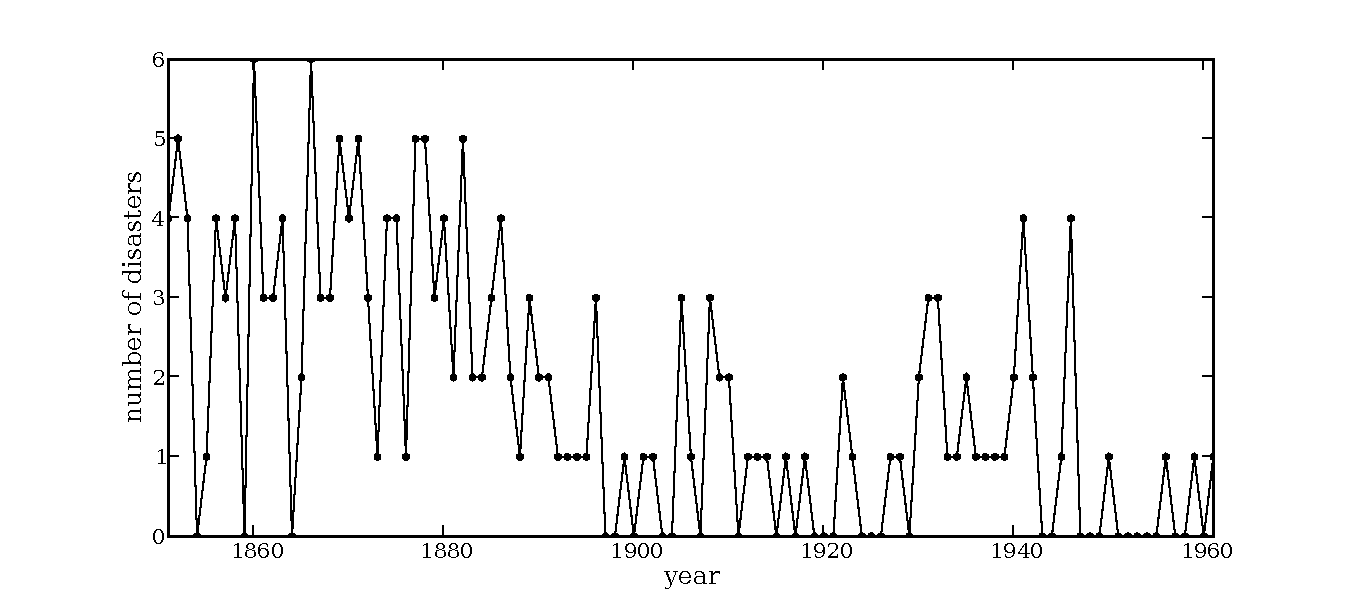
\epsfig{file=disasterts.pdf, width=15cm}
\end{center}
Occurrences of disasters in the time series is thought to be derived from a Poisson process with a large rate parameter in the early part of the time series, and from one with a smaller rate in the later part. We are interested in locating the change point in the series, which perhaps is related to changes in mining safety regulations.

We represent our conceptual model formally as a statistical model:
\begin{equation}
    \begin{array}{ccc}
        (D_t | s, e, l) \sim \textup{Po}\left(r_t\right), & r_t=\left\{\begin{array}{ll}
            e & t\le s\\ l & t>s
            \end{array}\right.,&t\in[t_l,t_h]\\
        s\sim \textup{U}(t_l, t_h)\\
        e\sim \textup{Exp}(r_e)\\
        l\sim \textup{Exp}(r_l)        
    \end{array}
    \label{disastermodel} 
\end{equation}
The symbols have the following meanings:
\begin{description}
    \item[$D_t$:] The number of disasters in year $t$.
    \item[$r_t$:] The rate parameter of the Poisson distribution of disasters in year $t$.
    \item[$s$:] The year in which the rate parameter changes.
    \item[$e$:] The rate parameter before the switchpoint $s$.
    \item[$l$:] The rate parameter after the switchpoint.
    \item[$t_l$ and $t_h$:] The lower and upper boundaries of time $t$.
    \item[$r_e$ and $r_l$:] Prior parameters.
\end{description}
Because we have defined $D$ by its dependence on $s$, $e$ and $l$, the latter three are known as the `parents' of $D$ and $D$ is called their `child'. Similarly, parents of $s$ are $t_l$ and $t_h$, and $s$ is the child of $t_l$ and $t_h$.

At the model-specification stage (before the data have been observed), $D$, $s$, $e$, $r$ and $l$ are all random variables. Under the Bayesian interpretation of probability, `random' variables have not necessarily arisen from a physical random process. `Random' only means that we are unsure of their values. Random variables are represented by class \texttt{Variable}, which has subclasses \texttt{Stochastic} and \texttt{Deterministic}.

There is a difference between $r$ and the other variables: if we knew the values of $r$'s parents, we could compute the value of $r$ with no uncertainty. This variable is defined by a mathematical function which returns its value given values for its parents. The \texttt{Deterministic} class represents such variables. This nomenclature is a bit confusing, because these objects usually represent random variables; if the parents of $r$ are random, $r$ is random also. If verbosity were not a problem, the best name for this class would probably be \texttt{DeterminedByValuesOfParents}.

On the other hand, even given values for the parents of $s$ we would still be uncertain of $s$'s value, and similarly for $D$, $e$ and $l$. These variables are defined by probability distributions that express how plausible their candidate values are given values for their parents. The \texttt{Stochastic} class represents these variables. The best name for these objects would probably be \texttt{RandomEvenGivenValuesOfParents}.
 

\section{The \texttt{Stochastic} class}

A stochastic variable has the following major attributes: 
\begin{description}
    \item[\texttt{value}:] The variable's current value.
    \item[\texttt{logp}:] The log-probability of the variable's current value given the values of its parents.
\end{description}
A stochastic variable can optionally be endowed with a method called \texttt{\bfseries random}, which draws a value for the variable given the values of its parents. Note that the \texttt{random} method does not provide a Gibbs sample unless the variable has no children.

A stochastic variable has the following additional attributes:
\begin{description}
    \item[\texttt{parents}:] A dictionary containing the variable's parents. The keys of the dictionary correspond to the names assigned to the variable's parents by the variable, and the values correspond to the actual parents. For example, the keys of $s$'s parents dictionary would be \texttt{t_l} and \texttt{t_h}. Thanks to Python's dynamic typing, parents may be of any class or type.
    \item[\texttt{children}:] A set containing the variable's children. This set is produced automatically; the user doesn't need to worry about filling it.
    \item[\texttt{extended_parents}:] A set containing all the stochastic variables on which the variable depends either directly or via an unbroken sequence of deterministic variables. If the value of any of these variables changes, the variable will need to recompute its log-probability.
    \item[\texttt{extended_children}:] A set containing all the stochastic variables and potentials that depend on the variable either directly or via an unbroken sequence of deterministic variables. If the variable's value changes, all of these variables will need to recompute their log-probabilities.
    \item[\texttt{coparents}:] A set containing all the stochastic variables that share extended children with the variable.
    \item[\texttt{moral_neighbors}:] A set containing the union of the variable's extended parents, extended children and coparents, with potentials removed.
    \item[\texttt{markov_blanket}:] A set containing self and self's moral neighbors.
    \item[\texttt{isdata}:] A boolean indicating whether the variable's value has been observed (is fixed).
    \item[\texttt{trace}:] The trace object assigned to the variable, see chapter \ref{chap:database}.
    \item[\texttt{__name__}:] The name of the variable, should be unique.
    \item[\texttt{__doc__}:] The docstring of the variable.
\end{description}

Subclasses of \texttt{Stochastic} include the \texttt{DiscreteStochastic} class, which represents integer-valued variables, and the \texttt{BinaryStochastic} class, which represents Bernoulli or indicator variables. 

\subsection{Instantiation of stochastic variables}
There are four ways to instantiate stochastic variables, called the `short', `long', `one-liner' and `direct' interfaces.
\begin{description}    
    \item[Short] Uniformly-distributed stochastic variable $s$ could be created as follows:
    \begin{verbatim}
@stoch
def s(value=1900, t_l=1851, t_h=1962):
    """The switchpoint for the rate of disaster occurrence."""
    if value > t_h or value < t_l:
        return -Inf
    else:
        return -log(t_h - t_l) 
    \end{verbatim}
    The \texttt{Stochastic} object produced by the decorator \texttt{stoch} will evaluate its log-probability using the function \texttt{s}. The \texttt{value} argument, which is required, provides an initial value for the variable. The names of the function \texttt{s}'s other arguments will become the keys of the stochastic variable \texttt{s}'s \texttt{parents} dictionary. The values of these arguments will become the values of the parents.

Stochastic variables may be valued as any object, their parents may be any objects, and there is absolutely no restriction on the log-probability function, as long as it returns a real number (float). PyMC, scientific Python and numerical Python all provide fast implementations of several standard probability distributions that can be used to create stochastic variables.

    The decorater \texttt{stoch} can take a flag called \texttt{trace} which signals to \texttt{MCMCSampler} instances whether an MCMC trace should be kept for the stochastic variable: \texttt{@stoch(trace = False)} would turn tracing off. Similarly, it can take an integer-valued argument called \texttt{verbose} that controls the amount of output the variable prints to the screen. The default is $0$, no output; the maximum value is 3.

    \item[Long] The long interface allows the user to specify a \texttt{random} method for sampling the stochastic variable's value conditional on its parents.
    \begin{verbatim}
@stoch
def s(value=1900, t_l=1851, t_h=1962):
    """The switchpoint for the rate of disaster occurrence."""

    def logp(value, t_l, t_h):
        if value > t_h or value < t_l:
            return -Inf
        else:
            return -log(t_h - t_l) 
            
    def random(t_l, t_h):
        return round( (t_l - t_h) * random() ) + t_l

    rseed = 1.
    \end{verbatim}
The stochastic variable again gets its name, docstring and parents from function s, but in this case it will evaluate its log-probability using the \texttt{logp} function. The \texttt{random} function will be used when \texttt{s.random()} is called. Note that it doesn't take a \texttt{value} argument, because it provides a new value. \textbf{XXX David explain rseed} \texttt{rseed} provides a seed for the RNG. The \texttt{value} argument is optional if a \texttt{random} method is provided; if no initial value is provided, it will be drawn using the \texttt{random} method.

\item[One-Liner] Stochastic variables with standard distributions (see chapter \ref{chap:distributions} ) can be instantiated in a single line using special subclasses of \texttt{Stochastic}. Exponentially-distributed variable $e$ could be instantiated using the one-liner interface as follows:
\begin{verbatim}
    e = Exponential('e', 1., beta = 1)
\end{verbatim}
You can use the class factory \texttt{stoch_from_dist} to produce \texttt{Stochastic} subclasses like \texttt{Exponential} from probability distributions not included with PyMC. These classes' init methods take the following arguments:
\begin{description}
    \item[\texttt{name}:] The name of the variable.
    \item[\texttt{value}:] An initial value for the variable.
    \item[\texttt{parents}:] Keyword arguments specifying the parents of the variable.
    \item[\texttt{isdata} (optional)]
    \item[\texttt{doc} (optional):] The docstring of the variable.
    \item[\texttt{verbose} (optional):] An integer from 0 to 3.
    \item[\texttt{trace} (optional):] A boolean indicating whether a trace should be kept for this variable in Monte Carlo fitting methods.
    \item[\texttt{cache_depth}:] See section \ref{sec:caching}. 
\end{description}


    \item[Direct] It's possible to instantiate \texttt{Stochastic} directly:
\begin{verbatim}
def s_logp(value, t_l, t_h):
    if value > t_h or value < t_l:
        return -Inf
    else:
        return -log(t_h - t_l) 

def s_rand(t_l, t_h):
    return round( (t_l - t_h) * random() ) + t_l

s = Stochastic( logp = s_logp, 
                name = 's', 
                value = 1900,
                parents = {'t_l': 1851, 't_h': 1962},
                doc = 'The switchpoint for the rate of disaster occurrence.',
                random = s_rand, 
                trace = True, 
                rseed = 1., 
                isdata = False,
                verbose = 0,
                cache_depth = 2)
\end{verbatim}
\end{description}

\subsection{Don't update stochastic variables' values in-place}\label{sub:warning}

\texttt{Stochastic} objects' values should not be updated in-place. This would confuse PyMC's caching scheme and corrupt the `last value' attribute, which is used for rejecting jumps. The only way a stochastic variable's value should be updated is using statements of the following form:
\begin{verbatim}
    A.value = new_value
\end{verbatim}
where \texttt{new_value} is an object that has just been created for this purpose. The following are in-place updates and should \emph{not} be used:
\begin{itemize}
    \item \texttt{A.value += 3}
    \item \texttt{A.value[2,1] = 5}
    \item \texttt{A.value.attribute = new_attribute_value}. This is an in-place update regardless of what type of object \texttt{A.value} is.
\end{itemize}

This restriction becomes onerous if a step method proposes values for the elements of an array-valued variable separately. In this case, it may be preferable to partition the variable into several variables stored in an array or list.

\section{Data}

Although the data $D$ was a random variable at the model-specification stage, we subsequently fixed its value by observing it. Such variables are represented by \texttt{Stochastic} objects whose \texttt{isdata} attribute is set to \texttt{True}. If a stochastic variable's \texttt{isdata} flag is \texttt{True}, its value cannot be changed.

\subsection{Why are data and unknown variables represented by the same object?}
Since it's represented by a \texttt{Stochastic} object, $D$ is defined by its dependence on its parents $s$, $e$ and $l$ even though its value is fixed. This isn't just a quirk of PyMC's syntax; Bayesian hierarchical notation itself makes no distinction between random variables and data. The reason is simple: to use Bayes' theorem to compute the posterior $p(e,s,l|D)$ of model \ref{disastermodel}, we need to use the likelihood $p(D|e,s,l)$. Even though $D$'s value is known and fixed, we need to formally assign it a probability distribution as if it were a random variable.

This point can be counterintuitive at first, as many peoples' instinct is to regard data as fixed a priori and unknown variables as dependent on the data. One way to understand this issue is to think of statistical models like (\ref{disastermodel}) as predictive models for data, or as models of the processes that gave rise to data. Before observing the value of $D$, we could have easily sampled from its prior predictive distribution $p(D)$ as follows:
\begin{enumerate}
    \item Sample $e$, $s$ and $l$ from their priors.
    \item Sample $D$ conditional on these values.
\end{enumerate}
Even after we observe the value of $D$, we need to use this process model to make inferences about $e$, $s$ and $l$; it's the only information we have about how the variables are related.

\medskip
To look at the issue another way, we could in principle have written a model equivalent to (\ref{disastermodel}) in such a way that $D$ depended on nothing and everything else depended on $D$, for example
\begin{eqnarray*}
    s|e,l,D\sim\cdot\\
    e|l,D\sim\cdot\\
    l|D\sim\cdot\\
    D=D_*
\end{eqnarray*}

This would have felt more natural in some ways, because we would have the unknown stochastic variables depending on the data. However, if we could write down that model using standard distributions we could trivially compute and sample from the posterior,
\begin{eqnarray*}
    p(s,e,l|D) = p(s|e, l, D) p(e|l, D) p(l|D),
\end{eqnarray*}
and we would have no use for MCMC or any other fitting method. Bayesian methods, and statistics in general, are needed when it's more natural to write down the data's dependence on the unknown variables than vice versa.

\subsection{Declaring stochastic variables to be data}

In the short and long interfaces, a \texttt{Stochastic} object's \texttt{isdata} flag can be set to true by stacking a \texttt{@data} decorator on top of the \texttt{@stoch} decorator:
\begin{verbatim}
@data
@stoch
def D(value = count_array, switchpoint = s, early_rate = e, late_rate = l):
    """The observed annual disaster counts."""
    logp = sum(-value[:switchpoint]) + early_rate * log(value[:switchpoint]) \
            - gammaln(early_rate))
    logp += sum(-value[switchpoint:] + late_rate * log(value[switchpoint:]) \
            - gammaln(late_rate))
    return logp
\end{verbatim}
In the one-liner and direct interfaces, the \texttt{isdata} argument can be simply set to \texttt{True}.


\section{The \texttt{Deterministic} class}\label{dtrm}

The \texttt{Deterministic} class represents variables whose values are fully determined by the values of their parents. In model (\ref{disastermodel}), $r$ can be represented as a deterministic variable. Recall that $r$ was defined by
\begin{eqnarray*}
    r_t=\left\{\begin{array}{ll}
        e & t\le s\\ l & t>s
        \end{array}\right.,
\end{eqnarray*}
so $r$'s value can be computed from the values of its parents $e$, $l$ and $s$.

A deterministic variable's most important attribute is \texttt{\bfseries value}, which gives the current value of the variable given the values of its parents. Like \texttt{Stochastic}'s \texttt{logp} attribute, this attribute is computed on-demand and cached for efficiency.

A Deterministic variable has the following additional attributes:
\begin{description}
    \item[\texttt{parents}:] A dictionary containing the variable's parents. The keys of the dictionary correspond to the names assigned to the variable's parents by the variable, and the values correspond to the actual parents. Thanks to Python's dynamic typing, parents may be of any class or type.
    \item[\texttt{children}:] A set containing the variable's children, which must be nodes. This set is produced automatically; the user doesn't need to worry about filling it.
    \item[\texttt{trace}:] The trace object assigned to the variable, see chapter \ref{chap:database}.
    \item[\texttt{__name__}:] The name of the variable, should be unique.
    \item[\texttt{__doc__}:] The docstring of the variable.
\end{description}
Deterministic variables have no methods.


\subsection{Instantiation of deterministic variables}
Deterministic variables are less complicated than stochastic variables, and there are only two ways to instantiate them:
\begin{description}
    \item[Decorator] A deterministic variable can be instantiated via a decorator in a way very similar to \texttt{Stochastic}'s short interface:
\begin{verbatim}
@dtrm
def r(switchpoint = s, early_rate = e, late_rate = l):
    """The rate of disaster occurrence."""
    value = zeros(N)
    value[:switchpoint] = early_rate
    value[switchpoint:] = late_rate
    return value
\end{verbatim}
The function supplied should return a new value (which may be any object) for the variable. Arguments' keys and values are converted into a parent dictionary as with \texttt{Stochastic}'s short interface. The function's \texttt{__name__} is passed on to the variable. The \texttt{dtrm} decorator can take \texttt{trace} and \texttt{verbose} arguments, like the \texttt{stoch} decorator.
    \item[Direct] The same variable could be instantiated directly as follows:
\begin{verbatim}
def r_eval(switchpoint = s, early_rate = e, late_rate = l):
    value = zeros(N)
    value[:switchpoint] = early_rate
    value[switchpoint:] = late_rate
    return value

r = Deterministic(  eval = r_eval, 
                    name = 'r',
                    parents = {'switchpoint': s, 'early_rate': e, 'late_rate': l}),
                    doc = 'The rate of disaster occurrence.',
                    trace = True,
                    verbose = 0,
                    cache_depth = 2)
\end{verbatim}
The \texttt{trace} flag signals to \texttt{Model} whether to keep a trace for the variable, as with stochastic variables.
\end{description}

Note that deterministic variables have no \texttt{isdata} flag. If a deterministic variable's value were known, its parents would be restricted to the inverse image of that value under the deterministic variable's evaluation function. This usage would be extremely difficult to support in general, but it can be implemented for particular applications at the \texttt{StepMethod} level.

\subsection{Deterministic variables are optional}
If we make a deterministic variable out of $r$, we'll want to rewrite $D$ as follows:
\begin{verbatim}
@data
@stoch
def D(value=count_array, rate=r):
    """The observed annual disaster counts."""
    return sum(-value + rate * log(value) - gammaln(rate))
\end{verbatim}
It's up to us whether to use $r$ explicitly or compute it implicitly in $D$'s logp function. However, deterministic variables can be nice for the following reasons:
\begin{itemize}
    \item They can save code duplication,    
    \item they can be computationally efficient (because they save code duplication), and
    \item sometimes it's convenient to produce a dynamic trace of the value of a function of stochastic variables.
\end{itemize}

\section{Using \texttt{Variables} as parents of \texttt{Variables}}

Let's take a closer look at our most recent definition of $D$:
\begin{verbatim}
@data
@stoch
def D(value=count_array, rate=r):
    """The observed annual disaster counts."""
    return sum(-value + rate * log(value) - gammaln(rate))
\end{verbatim}
The value of argument \texttt{rate} is a \texttt{Deterministic} object, not a number. Why aren't errors raised when we attempt to multiply \texttt{rate} by an array?

Whenever a variable is used as a parent for a child variable, it is replaced with its \texttt{value} attribute when the child's value or log-probability is computed. When $D$'s log-probability is recomputed, \texttt{r.value} is passed to the function as argument \texttt{rate}. To see the values of the parents of $D$, look at \texttt{D.parents.value}.

\section{Containers (optional)}\label{sub:container}
In the following situation, it would be inconvenient to assign a unique label to each parent of $y$:
\begin{eqnarray*}
    x_0 \sim \textup N(0,\tau_x)\\
    x_{i+1}|x_i\sim\textup{N}(x_i, \tau_x),& i=0\ldots N-2\\
    y|x \sim \textup N\left(\sum_{i=0}^{N-1}x_i^2,\tau_y\right).
\end{eqnarray*}
$y$ depends on every element of the Markov chain $x$, but we wouldn't want to manually enter $N$ parent labels \texttt{'x_0'}, \texttt{'x_1'}, etc.

This situation can be handled in the natural way:
\begin{verbatim}
@stoch
def x_0(value=0, mu = 0, tau = 1):
    return normal_like(value, mu, tau)

x = [x_0]
last_x = x_0

for i in range(1,N):          
    @stoch
    def x_now(value=0, mu = last_x, tau = 1):
        return normal_like(value, mu, tau)
        
    last_x = x_now
    
    x.append(x_now)

@data
@stoch
def y(value = 1, mu = x, tau = 100):
    mu_sum = 0
    for i in range(N):
        mu_sum += mu[i] ** 2
    return normal_like(value, mu_sum, tau)
\end{verbatim}
The list \texttt{x} is transparently wrapped in an appropriate container class by the function \texttt{Container}.

Containers, like variables, have an attribute called \texttt{value}. This attribute returns a copy of the (possibly nested) iterable that was passed into the container function, but with each variable inside replaced with \emph{its} value. 

Containers can currently be constructed from lists, tuples, dictionaries, numpy arrays, modules, sets and any object with a \texttt{__dict__} attribute. Variables and non-variables can be freely mixed in these iterables, and different types of iterables can be nested. Containers attempt to behave like the iterables they wrap. All containers are subclasses of \texttt{ContainerBase}. 

Nodes whose parents are containers make private (shallow) copies of those containers on instantiation. This is done for technical reasons rather than to protect users from accidental misuse.

Containers have the following useful attributes in addition to \texttt{value}:
\begin{itemize}
    \item\texttt{variables}
    \item\texttt{stochs}
    \item\texttt{potentials}
    \item\texttt{dtrms}
    \item\texttt{data}
    \item\texttt{step_methods}.
\end{itemize}
Each of these attributes is a set containing all the objects of each type in a container, and within any containers in the container.

\section{The \texttt{Potential} class}


The joint density corresponding to model (\ref{disastermodel}) can be written as follows:
\begin{eqnarray*}
    p(D,s,l,e) = p(D|s,l,e) p(s) p(l) p(e).
\end{eqnarray*}
Each factor in the joint distribution is a proper, normalized probability distribution for one of the variables conditional on its parents. Such factors are contributed by \texttt{Stochastic} objects.

In some cases, it's nice to be able to modify the joint density by incorporating terms that don't correspond to probabilities of variables conditional on parents, for example:
\begin{eqnarray*}
    p(x_0, x_2, \ldots x_{N-1}) \propto \prod_{i=0}^{N-2} \psi_i(x_i, x_{i+1}).
\end{eqnarray*}
Arbitrary factors such as $\psi$ are contributed by objects of class \texttt{Potential} (\cite{dawidmarkov} and \cite{jordangraphical} call these terms `factor potentials'). Bayesian hierarchical notation (cf model (\ref{disastermodel})) doesn't accomodate these potentials. However, they are useful for certain cases where there is no natural dependence hierarchy, especially Markov random fields.

% Even when there is a definite dependence hierarchy, potentials can provide a useful shorthand. Consider a new example: we have a dataset $t$ consisting of the days on which several marked animals were recaptured. We believe that the probability $S$ that an animal is not recaptured on any given day can be explained by a covariate vector $x$. We model this situation as follows:
% \begin{eqnarray*}
%     t_i|S_i \sim \textup{Geometric}(S_i), & i=1\ldots N\\
%     S_i = \textup{logit}^{-1}(\beta x_i), &i=1\ldots N\\
%     \beta\sim \textup{N}(\mu_\beta, V_\beta).
% \end{eqnarray*}
% So far, so good. Now suppose we have some knowledge of other related experiments and we have a good idea of what $S$ will be before seeing the data. It's not obvious how to work this prior information in, because as we've written the model $S$ is completely determined by $\beta$. There are three options within the strict Bayesian hierarchical framework:
% \begin{itemize}
%     \item Work the prior information into the prior on $\beta$.
%     \item Incorporate the data from the previous experiments explicitly into the model.
%     \item Refactor the model so that $S$ is at the bottom of the hierarchy, and assign the prior directly.
% \end{itemize}
% 
% Factor potentials provide a convenient way to incorporate the prior information without the need for such major modifications. We can simply modify the joint distribution from
% \begin{eqnarray*}
%     p(t|S(x,\beta)) p(\beta)
% \end{eqnarray*}
% to
% \begin{eqnarray*}
%     \gamma(S,a,b) p(t|S(x,\beta)) p(\beta),
% \end{eqnarray*}
% where $\gamma$ expresses the prior information. It's a good idea to check the induced priors on $S$ and $\beta$ for sanity. This can be done in PyMC by fitting the model with the data $t$ commented out.

\bigskip
Potentials have one important attribute, \texttt{\bfseries logp}, which gives the log of their current probability or probability density value given the values of their parents. They have the following additional attributes:
\begin{description}
    \item[\texttt{parents}:] A dictionary containing the potential's parents. The keys of the dictionary correspond to the names assigned to the potential's parents by the potential, and the values correspond to the actual parents. Thanks to Python's dynamic typing, parents may be of any class or type.
    \item[\texttt{__name__}:] The name of the potential, should be unique.
    \item[\texttt{__doc__}:] The docstring of the potential.
\end{description}
Potentials have no methods. They have no \texttt{trace} attribute, because they are not variables. They cannot serve as parents of variables for the same reason, so they have no \texttt{children} attribute.


\subsection{Instantiation of potentials}
There are two ways to instantiate potentials:
\begin{description}
    \item[Decorator] A potential can be instantiated via a decorator in a way very similar to \texttt{Stochastic}'s short interface and \texttt{Deterministic}'s decorator interface:
\begin{verbatim}
@potential
def psi_i(x_lo = x[i], x_hi = x[i+1]):
    """A pair potential"""
    return -(xlo - xhi)**2
\end{verbatim}
The function supplied should return a floating-point value. Arguments' keys and values are converted into a parent dictionary as with stochastic variable's medium interface. The function's \texttt{__name__} is passed on to the potential. The \texttt{potential} decorator can take \texttt{verbose} and \texttt{cache_depth} arguments like the \texttt{stoch} decorator.
    \item[Direct] The same potential could be instantiated directly as follows:
\begin{verbatim}
def psi_i_logp(x_lo = x[i], x_hi = x[i+1]):
    return -(xlo - xhi)**2
        
psi_i = Potential(  logp = psi_i_logp, 
                    name = 'psi_i',
                    parents = {'xlo': x[i], 'xhi': x[i+1]},
                    doc = 'A pair potential',
                    verbose = 0,
                    cache_depth = 2)
\end{verbatim}
\end{description}

\section{Graphing models (optional)}
\label{sec:graphical}

It's often helpful to view probability models graphically; graphical representations harmonize very well with object-oriented programming, so most Bayesian statistics packages (including PyMC) are at least somewhat graphically inspired. The function \texttt{graph} draws graphical representations of \texttt{Model} (chapter \ref{modelfitting}) instances using GraphViz via the Python package PyDot. See \cite{dawidmarkov} and \cite{jordangraphical} for more discussion of useful information that can be read off of graphical models. Note that these authors do not consider deterministic variables.

The symbol for stochastic variables is an ellipse. Parent-child relationships are indicated by arrows. These arrows point from parent to child and are labeled with the names assigned to the parents by the children. A graphical representation of model \ref{disastermodel} follows:
\begin{center}
    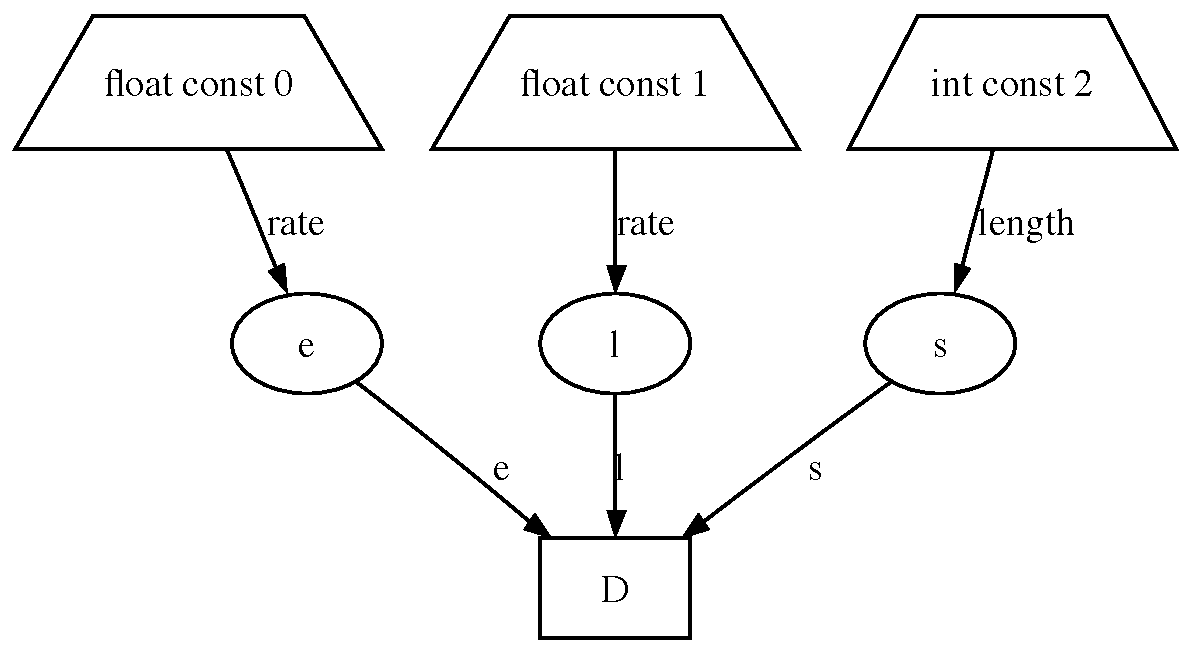
\epsfig{file=DisasterModel.pdf, width=6cm} 
\end{center} 
$D$ is shaded because it is flagged as data.

PyMC's symbol for deterministic variables is a downward-pointing triangle. A graphical representation of model \ref{disastermodel} with $r$ explicit follows:
\begin{center}
    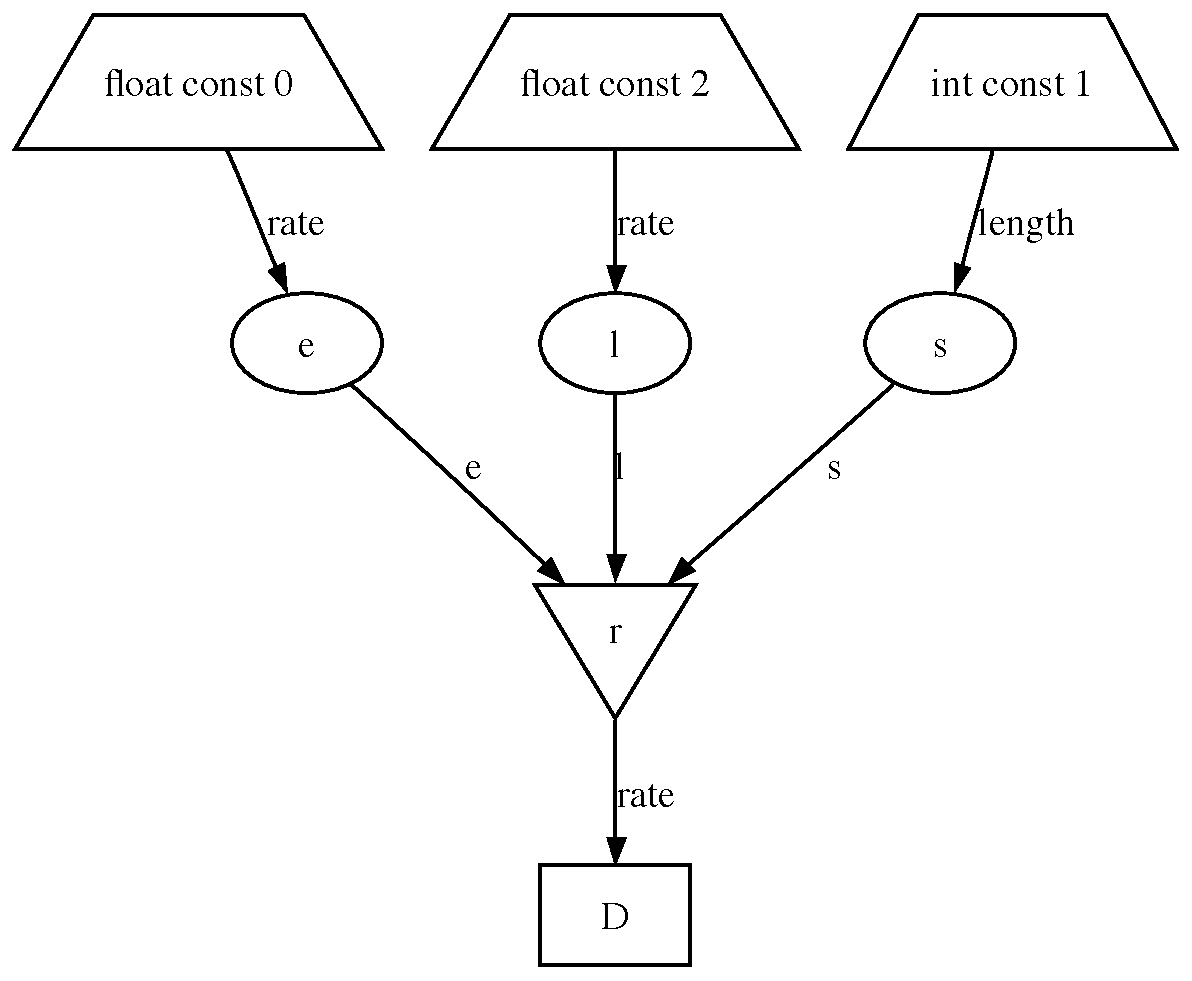
\epsfig{file=DisasterModel2.pdf, width=6cm} 
\end{center}
% Note that if a deterministic variable has more than one child, its parents each inherit all of its children when it is made implicit:
% \begin{center}
%     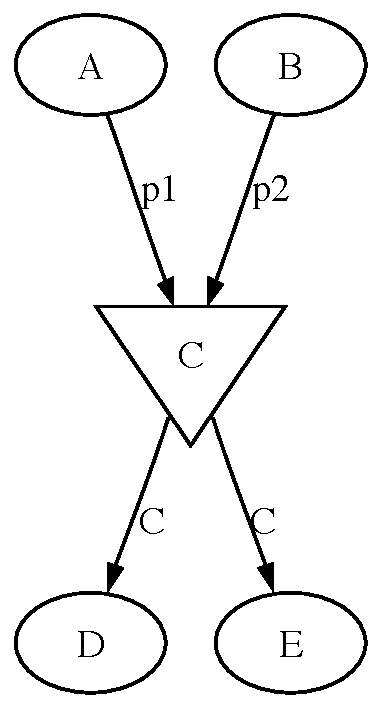
\epsfig{file=DeterministicPreInheritance.pdf, width=3.5cm} $\Rightarrow$ 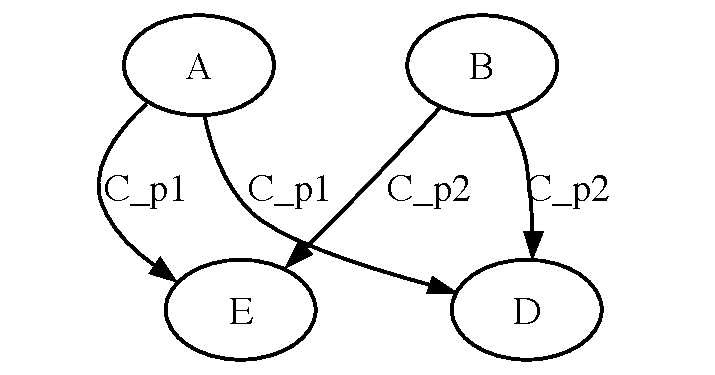
\epsfig{file=DeterministicPostInheritance.pdf, width=5cm}
% \end{center}
% These inherited children can be accessed via the \texttt{extended_children} attributes of the parents.

The symbol for factor potentials is a rectangle:
\begin{center}
    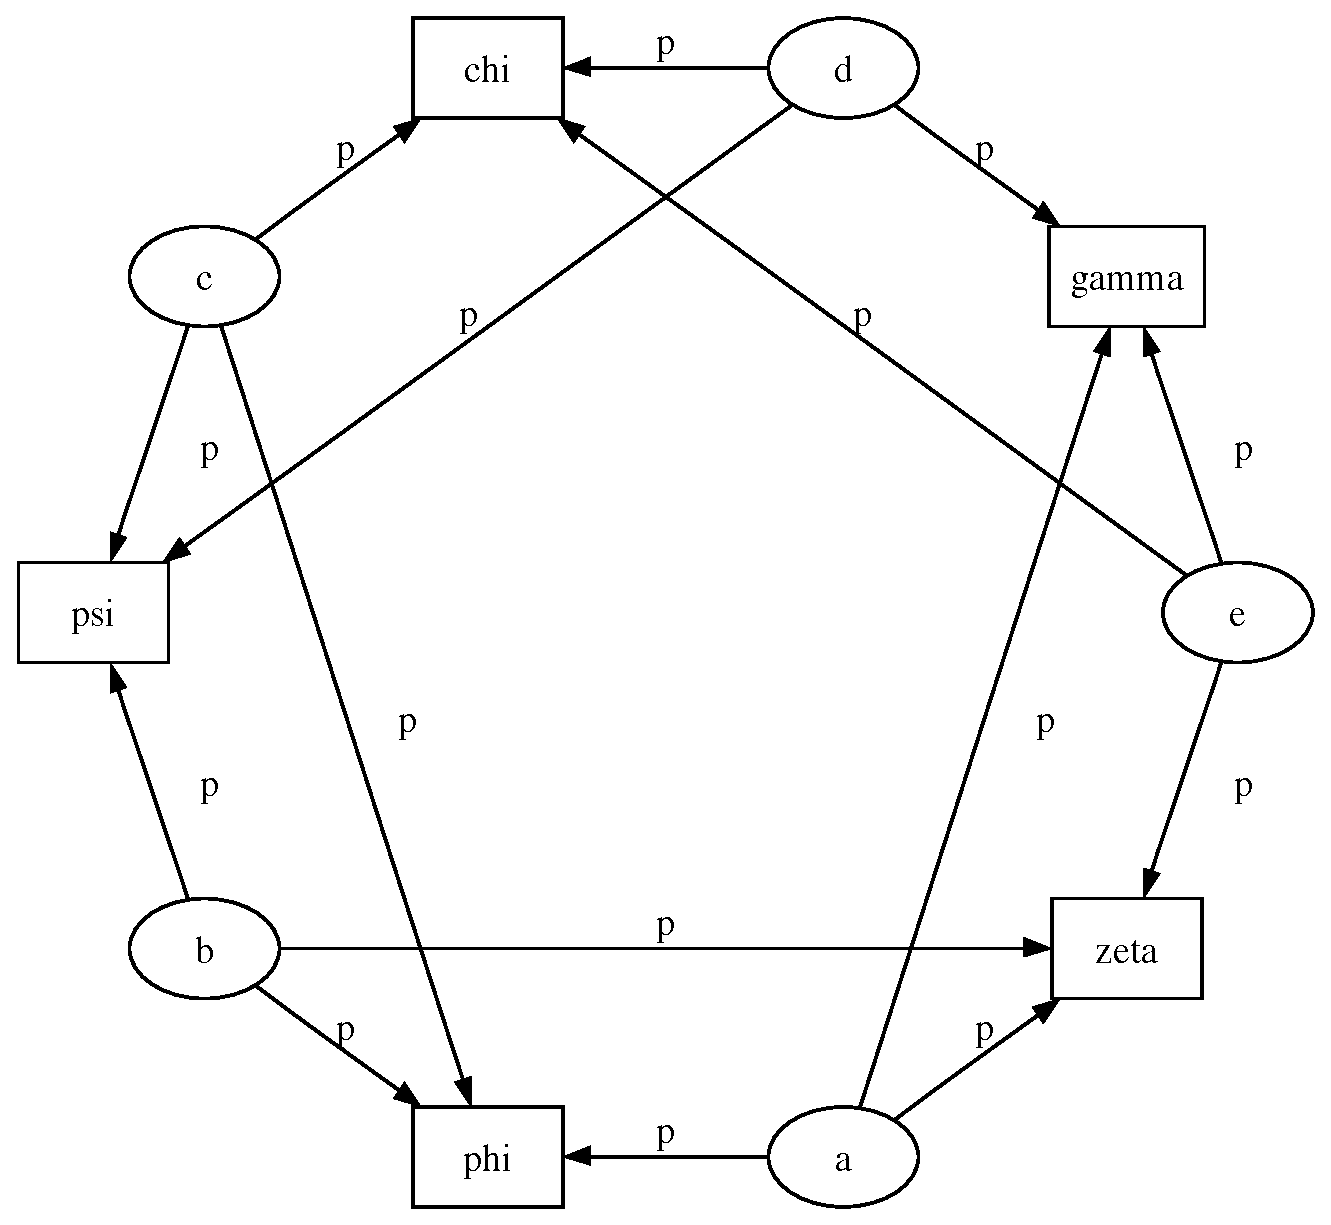
\epsfig{file=PotExample.pdf, width=10cm} 
\end{center}
Potentials are usually associated with \emph{undirected} grahical models. In undirected representations, each parent of a potential is connected to every other parent by an undirected edge:
\begin{center}
    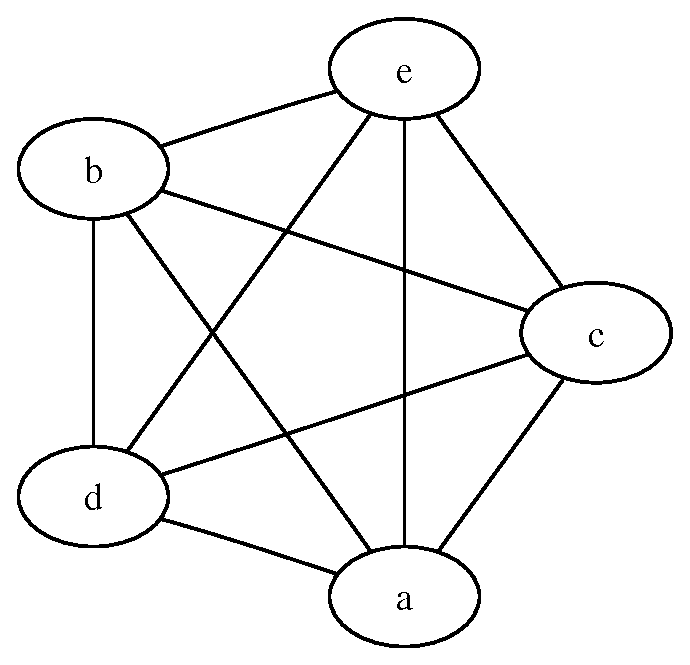
\epsfig{file=PotExampleCollapsed.pdf, width=5cm}
\end{center}

Directed or mixed graphical models can be represented in an undirected form by `moralizing', which is done by the function \texttt{moral_graph}.

\section{Class \texttt{LazyFunction} and caching (optional)}
\label{sec:caching} 

The \texttt{logp} attributes of stochastic variables and potentials and the \texttt{value} attributes of deterministic variables are wrappers for instances of class \texttt{LazyFunction}. Lazy functions are wrappers for ordinary Python functions. A lazy function \texttt{L} could be instantiated from a function \texttt{fun} as follows:
\begin{verbatim}
L = LazyFunction(fun, arguments)
\end{verbatim}
The argument \texttt{arguments} is a dictionary container (see section \ref{sub:container}); \texttt{fun} must accept keyword arguments only. When \texttt{L}'s \texttt{get()} method is called, the return value is the same as the call 
\begin{verbatim}
fun(**arguments.value)
\end{verbatim}
Note that no arguments need to be passed to \texttt{L.get}; lazy functions memorize their arguments.

Before calling \texttt{fun}, \texttt{L} will check the values of \texttt{arguments.variales} against an internal cache. This comparison is done \emph{by reference}, not by value, and this is the reason why stochastic variables' values cannot be updated in-place. If \texttt{arguments.variables}' values match a frame of the cache, the corresponding value is returned and \texttt{fun} is not called. If a call to \texttt{fun} is needed, \texttt{arguments.variables}' values and the return value are added to the cache. The oldest frame in the cache is removed. The depth of the cache can be set using the optimal init argument \texttt{cache_depth}, which defaults to 2.

Caching is helpful in MCMC, because variables' log-probabilities and values tend to be queried multiple times for the same parental value configuration. The default cache depth of 2 turns out to be most useful in Metropolis-Hastings-type algorithms involving proposed values that may be rejected.

Lazy functions are implemented in C via Pyrex.